\section{Программный пакет \texttt{NuPropagator}}
\label{sec:nupropagator}
\subsection{Структура программы}
\texttt{NuPropagator}~\cite{nupropagator2022} — модуль для моделирования распространения потоков нейтрино через вещество, в частности сквозь Землю, с учётом взаимодействий с обменом $W$ и $Z$ бозонами. 
\texttt{NuPropagator} реализован на языке \texttt{Python3} и распространяется через платформу \texttt{PyPI}, обеспечивая простую установку и интеграцию в существующие симуляционные цепочки.

Структура \texttt{NuPropagator} представлена на рис.~\ref{fig:nupropagator1}, на котором приведены соответствующие вспомогательные модули.
\begin{figure}[!h]
\centering
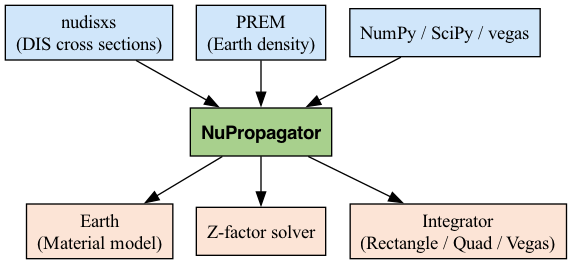
\includegraphics[width=\linewidth]{images/nupropagator_diagram.png}
\caption{Структура программного пакета \texttt{NuPropagator} и его зависимости.}
\label{fig:nupropagator1}
\end{figure}

В расчётах используются сечения взаимодействия нейтрино с нуклонами, предоставляемые пакетом \texttt{nudisxs}, описанными в разделах~\ref{sec:dis},\ref{sec:nudisxs}, модель плотности Земли PREM (приложение~\ref{sec:prem}) и   $\mathcal{Z}$-факторный метод, коротко изложенный в разделе~\ref{sec:zfactor}. Изотопный состав вещества задаётся в модуле \texttt{Earth}. Численное вычисление глубины использует несколько методов: квадратуры из пакета \texttt{SciPy.quad}, Монте-Карло \texttt{vegas}. \texttt{NuPropagator} учитываtn как поглощение, так и регенерацию потоков за счёт взаимодействий нейтрино с обменом $Z$ бозоном.

\texttt{NuPropagator} может использоваться как самостоятельный инструмент или как часть общего фреймворка, например, \texttt{NTSim}, разработанного для нейтринного телескопа Baikal-GVD~\cite{ntsim2025}. 
Он взаимодействует с генераторами событий, моделями детектора и другими компонентами цепочки симуляции, обеспечивая единое моделирование распространения нейтрино от источника до регистрации.

\subsection{Валидация \texttt{NuPropagator}}
Валидация \texttt{NuPropagator} выполнена сравнением с результатами  пакета \texttt{nuFATE}~\cite{Vincent_2017}, также решающим задачу транспорта нейтрино через Землю. Рассмотрим поток мюонных нейтрино, достигающих условную точку наблюдения,  расположенную на глубине 1~км от поверхности. Изучим потоки как функция энергии нейтрино и угла прихода. Для простоты зададим на поверхности Земли энергетический спектр  нейтрино в виде $F_0(E) \propto E^{-2}$.  

Потоки, вычисленные с помощью \texttt{NuPropagator} и \texttt{nuFATE}, обозначим как $F_\nu^{(1)}$ и $F_\nu^{(2)}$, соответственно. 
Для количественной оценки различий введена асимметрия
\begin{equation}
\delta_{\text{asym}} = 
2\,\frac{F_\nu^{(1)}(E, x) - F_\nu^{(2)}(E, x)}
       {F_\nu^{(1)}(E, x) + F_\nu^{(2)}(E, x)}.
\end{equation}

\begin{figure}[!h]
\centering
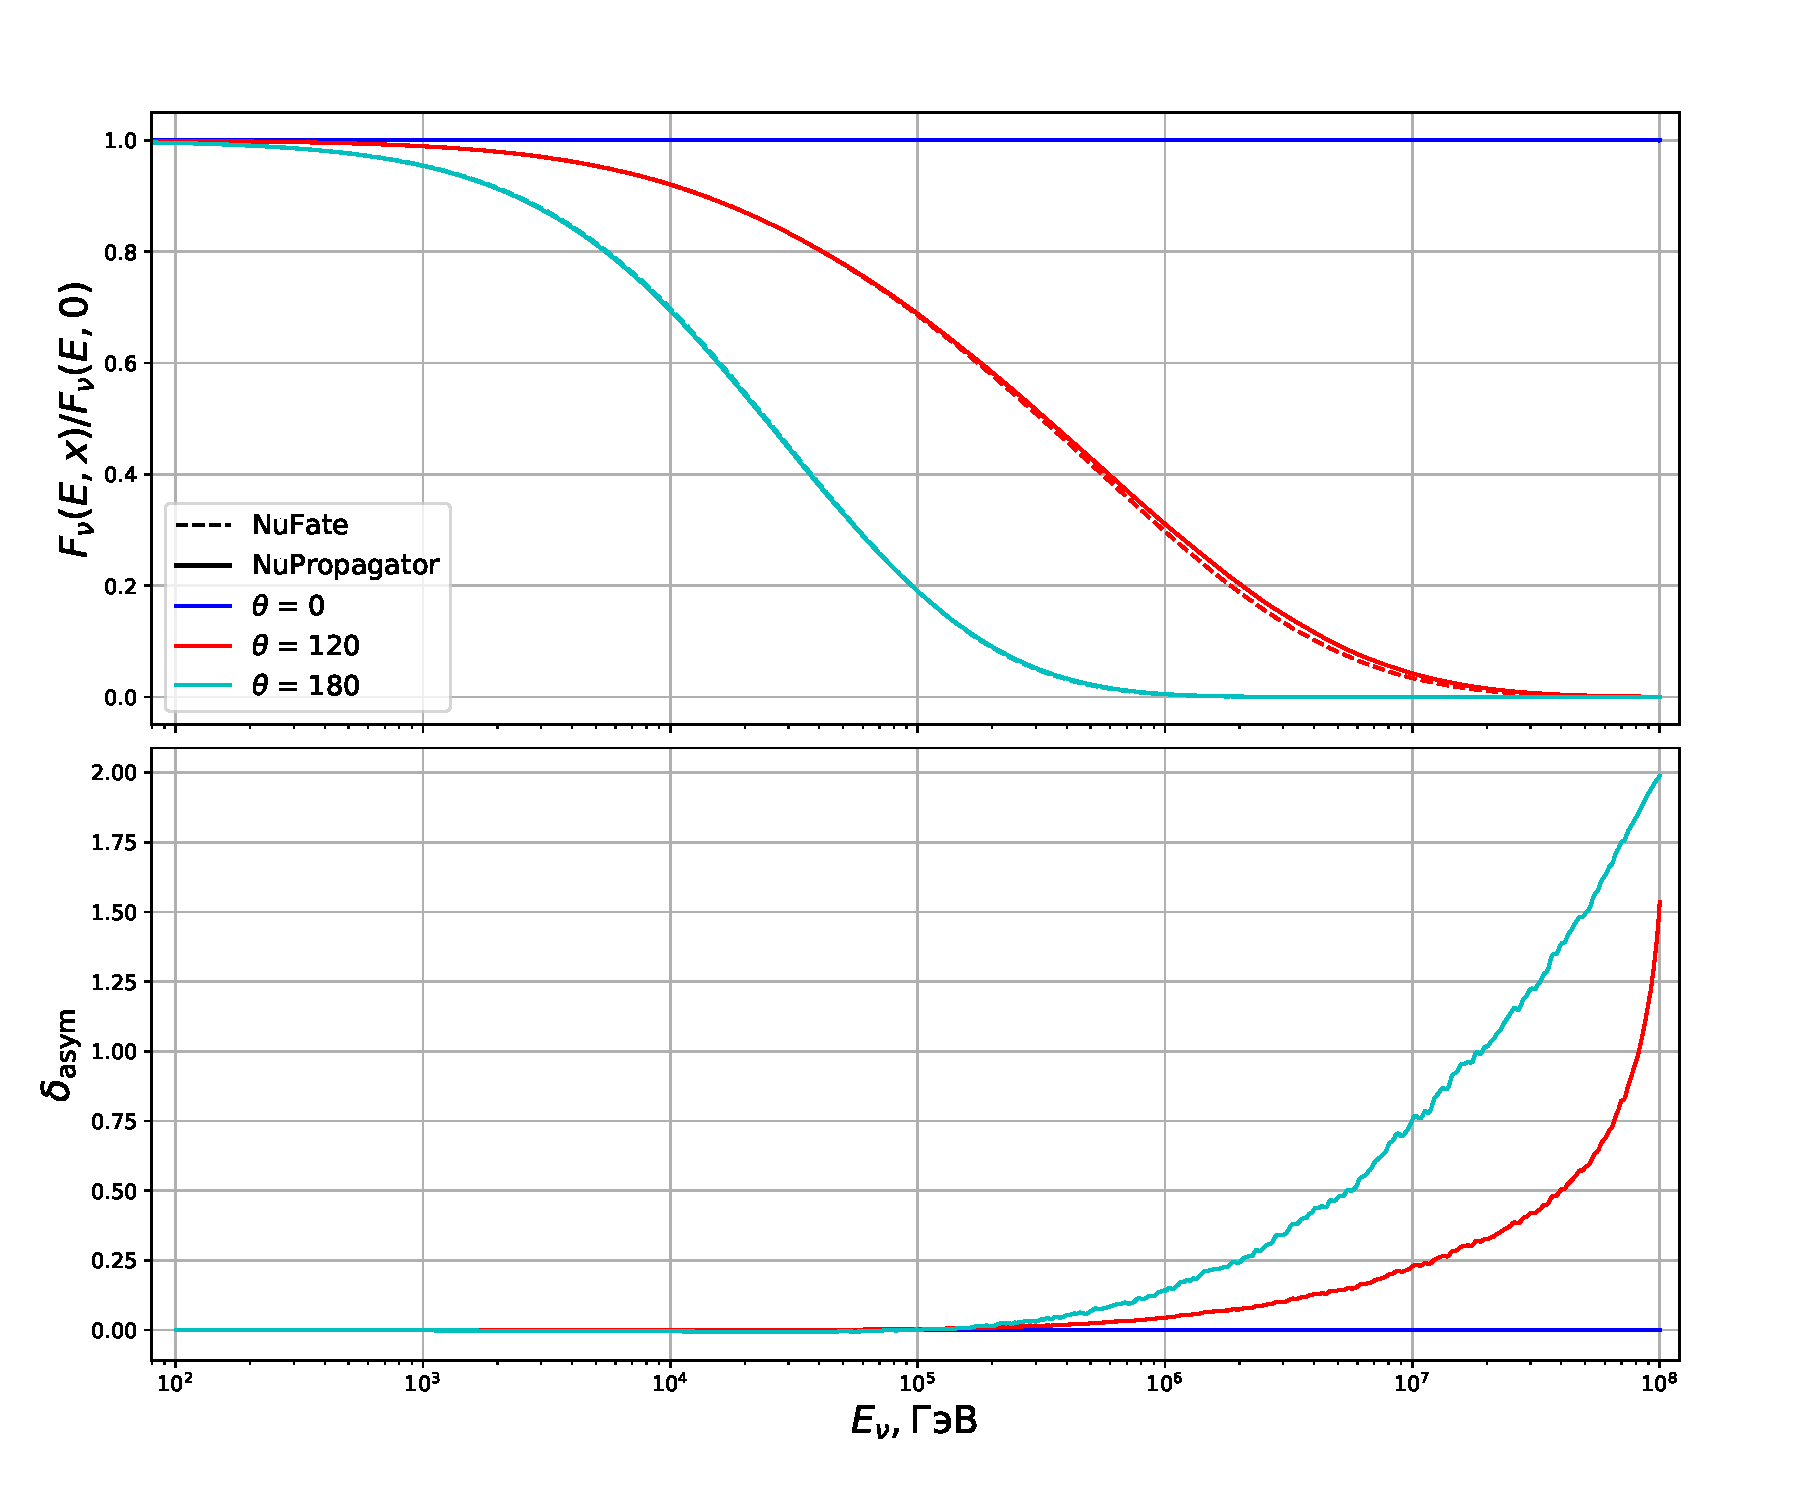
\includegraphics[width=0.8\linewidth]{images/NuProp/compNuandNu.pdf}
\caption{Сравнение потоков нейтрино, рассчитанных с помощью \texttt{NuPropagator} и \texttt{nuFATE}, при различных зенитных углах.}
\label{fig:flux_compare}
\end{figure}

Как видно из рис.~(\ref{fig:flux_compare}), оба расчёта дают близкие результаты при энергиях $E_\nu \lesssim 10^6$~ГэВ, которые согласуются в рамках неопределенности вычисления сечения глубоконеупругого рассеяния нейтрино на нуклоне. 
